\section{Results}
\label{sec:results}

\subsection{Background estimate from the ABCD method}
\label{sec:abcdres}

We begin by applying the ABCD method to estimate the background in the 2010 signal region.
The data yields in the four regions are summarized in Tables~\ref{tab:datayield1} and
the $y$ vs. \Ht\ distributions are displayed in Fig.~\ref{fig:abcdData1}.
The ABCD background prediction is $N_A \times N_C / N_B = 12.7 \pm 2.4$ (stat), in
agreement with the MC expectation. We also apply the ABCD' method to estimate the
background in this region, following the procedure of App.~\ref{app:abcdprime},
and find a predicted background of $12.8 \pm 2.9$ (stat), in good agreement
with the ABCD prediction.

Next, we apply the ABCD' method to predict the yields in the high \met\ and high \Ht\
signal regions. The $y$ vs. \Ht\ distributions for data are displayed in 
Fig.~\ref{fig:abcdprimedata}. The signal regions are indicated, as well as the control 
regions used to measure the $f(y)$ and $g(H_T)$ distributions. For the high \met\
signal region, we find a predicted yield of $1.0 \pm 0.3$ (stat), in reasonable
agreement with the MC prediction. For the high \Ht\ signal region, we do not find
any events in the control region used to extract $g(H_T)$ with \Ht\ $>$ 600 GeV,
and the ABCD' background estimate is therefore 0. To assess the statistical uncertainty
in this prediction, we add a single event ``by hand'' to the $g(H_T)$ distributiion
at $H_T = 600$ GeV, leading to a predicted yield of 0.6. 
%{\bf NEED TO THINK ABOUT THIS. THE PREDICTION DEPENDS ON WHERE IN HT YOU PUT THIS }
%{\bf SINGLE EVENT. FOR EXAMPLE, PUTTING IT AT 1000 GIVES A PREDICTION OF 1.2      }
%{\bf HOPEFULLY WITH ~3X MORE STATS WE WON'T BE IN THIS SITUATION                  }
These results are summarized in Table~\ref{tab:abcdprime}.

\begin{table}[hbt]
\begin{center}
\caption{\label{tab:abcdprime} 
Summary of results of the ABCD' method, applied to the 3 signal regions. The correction
factors are given in Table~\ref{tab:cor}.
}
\vspace{.25cm}
\begin{tabular}{lccccc}
\hline
Signal Region             &     ABCD' pred      &  correction factor  &  prediction                                  \\ 
\hline
2010 signal region        &  $12.8 \pm 2.9$     & $1.0 \pm 0.2$      & 12.8 $\pm$ 2.9 (stat) $\pm$ 2.6 (syst)        \\
high \met\ signal region  &  $1.0  \pm 0.3$     & $1.2 \pm 0.5$      &  1.2 $\pm$ 0.4 (stat) $\pm$ 0.5 (syst)        \\
high \Ht\ signal region   &  $0.0  \pm 0.6$     & $1.0 \pm 0.5$      &  0.0 $\pm$ 0.6 (stat) $\pm$ 0.3 (syst)        \\
\hline
\end{tabular}
\end{center}
\end{table}

\begin{figure}[tbh]
\begin{center}
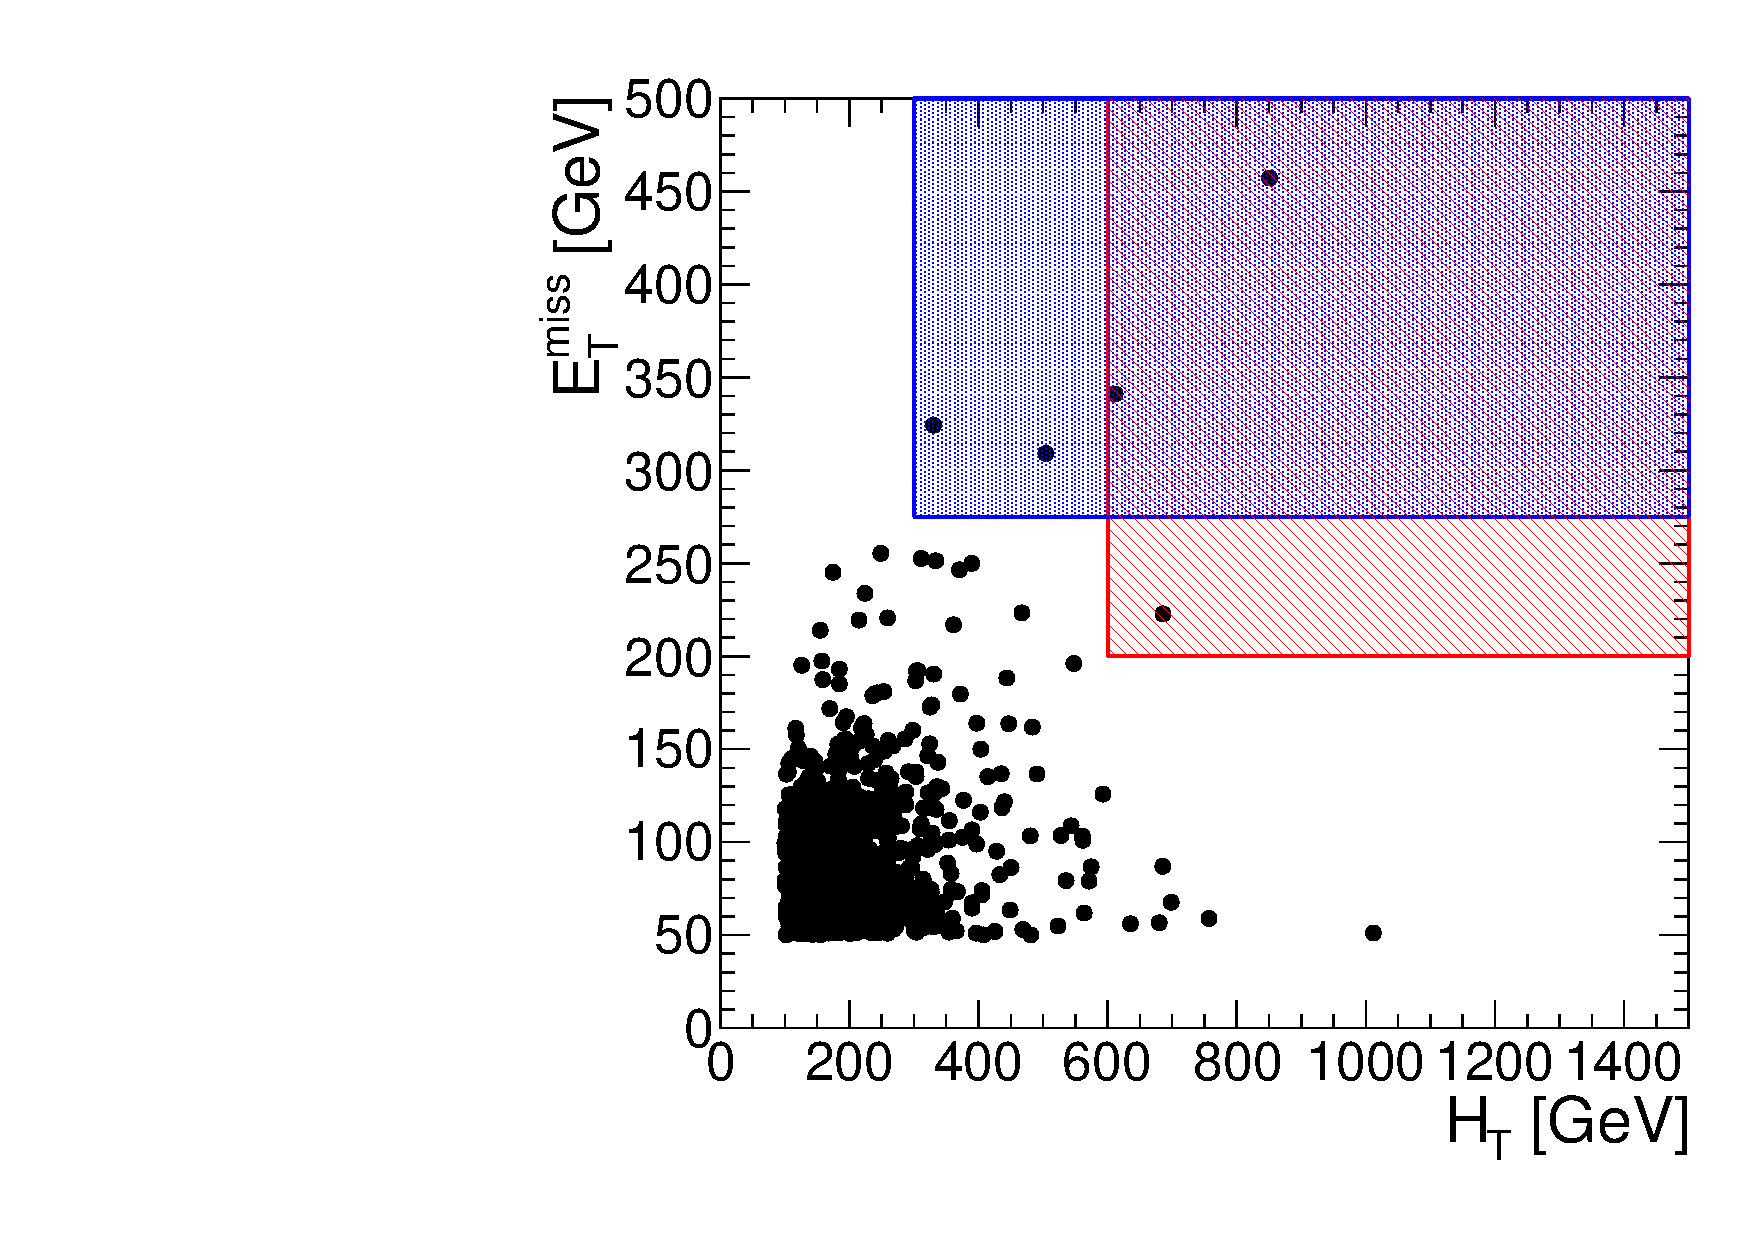
\includegraphics[width=0.48\linewidth]{plots/met_ht_349pb.pdf}
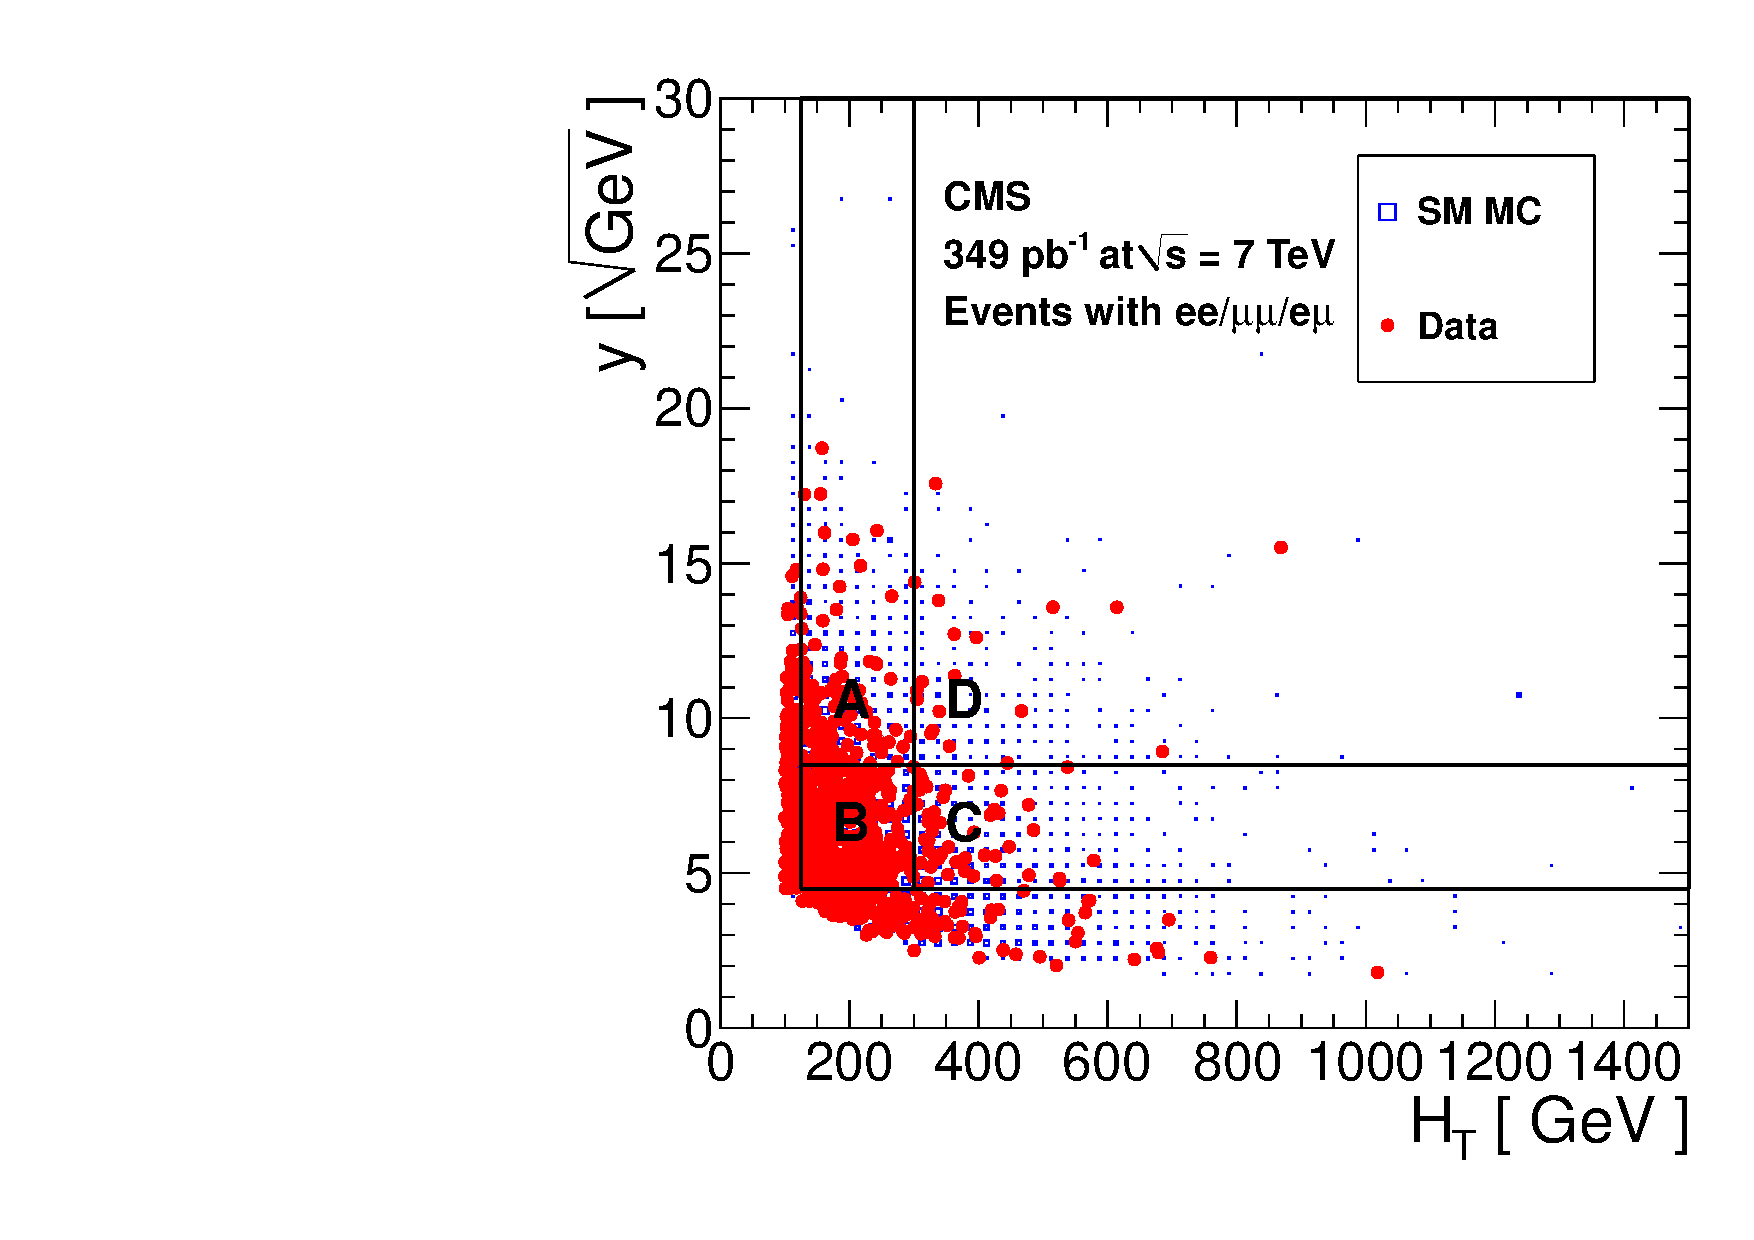
\includegraphics[width=0.48\linewidth]{plots/abcd_349pb.pdf}
\caption{\label{fig:abcdData1}\protect 
Left: Distribution of \met vs. \Ht\ for SM Monte Carlo and data. The 2011 high \Ht\ signal region is shown
in red. The 2011 high \met signal region is shown in blue.
Right: Distributions of $y$ vs. \Ht\ for SM Monte Carlo and data. The 2010 signal region boundaries are overlayed.}
\end{center}
\end{figure}

\begin{table}[h!]
\begin{center}
\caption{\label{tab:datayield1} 
Data yields in the four
regions of Figure~\ref{fig:abcdData1} for the 2010 signal region, 
as well as the predicted yield in region D given
by $N_A \times N_C / N_B$.  The quoted uncertainty
on the prediction in data is statistical only, assuming Gaussian errors.
We also show the SM Monte Carlo expectations with statistical errors only.
}
\vspace{.25cm}
\begin{tabular}{l||c|c|c|c||c}
\hline
           sample  &            $N_A$  &            $N_B$  &            $N_C$  &             $N_D$  &   $N_A \times N_C / N_B$ \\
\hline
            \ttll  & 63.9  $\pm$  2.0  &252.3  $\pm$  4.1  & 43.3  $\pm$  1.7  &  8.5  $\pm$  0.7  & 11.0  $\pm$  0.6        \\
           \tttau  & 18.5  $\pm$  1.1  & 55.9  $\pm$  1.9  & 10.3  $\pm$  0.8  &  3.4  $\pm$  0.5  &  3.4  $\pm$  0.4        \\
          \ttfake  &  1.0  $\pm$  0.3  &  6.6  $\pm$  0.7  &  1.1  $\pm$  0.3  &  0.4  $\pm$  0.2  &  0.2  $\pm$  0.1        \\
               DY  &  0.9  $\pm$  0.6  & 13.9  $\pm$  2.6  &  1.3  $\pm$  0.8  &  1.7  $\pm$  1.0  &  0.1  $\pm$  0.1        \\
              \WW  &  1.1  $\pm$  0.1  &  2.7  $\pm$  0.2  &  0.2  $\pm$  0.1  &  0.3  $\pm$  0.1  &  0.1  $\pm$  0.0        \\
              \WZ  &  0.1  $\pm$  0.0  &  0.6  $\pm$  0.0  &  0.1  $\pm$  0.0  &  0.0  $\pm$  0.0  &  0.0  $\pm$  0.0        \\
              \ZZ  &  0.0  $\pm$  0.0  &  0.2  $\pm$  0.0  &  0.0  $\pm$  0.0  &  0.0  $\pm$  0.0  &  0.0  $\pm$  0.0        \\
       single top  &  3.3  $\pm$  0.2  &  9.6  $\pm$  0.3  &  0.4  $\pm$  0.1  &  0.1  $\pm$  0.0  &  0.1  $\pm$  0.0        \\
           \wjets  &  1.0  $\pm$  1.0  &  2.2  $\pm$  1.1  &  0.0  $\pm$  0.0  &  0.0  $\pm$  0.0  &  0.0  $\pm$  0.0        \\
\hline
      Total SM MC  & 89.9  $\pm$  2.6  &344.0  $\pm$  5.3  & 56.6  $\pm$  2.1  & 14.5  $\pm$  1.4  & 14.8  $\pm$  0.7        \\
\hline
             data  &              110  &              381  &               44  &               19  & 12.7  $\pm$  2.4        \\
\hline
\end{tabular}
\end{center}
\end{table}


\begin{figure}[hbt]
\begin{center}
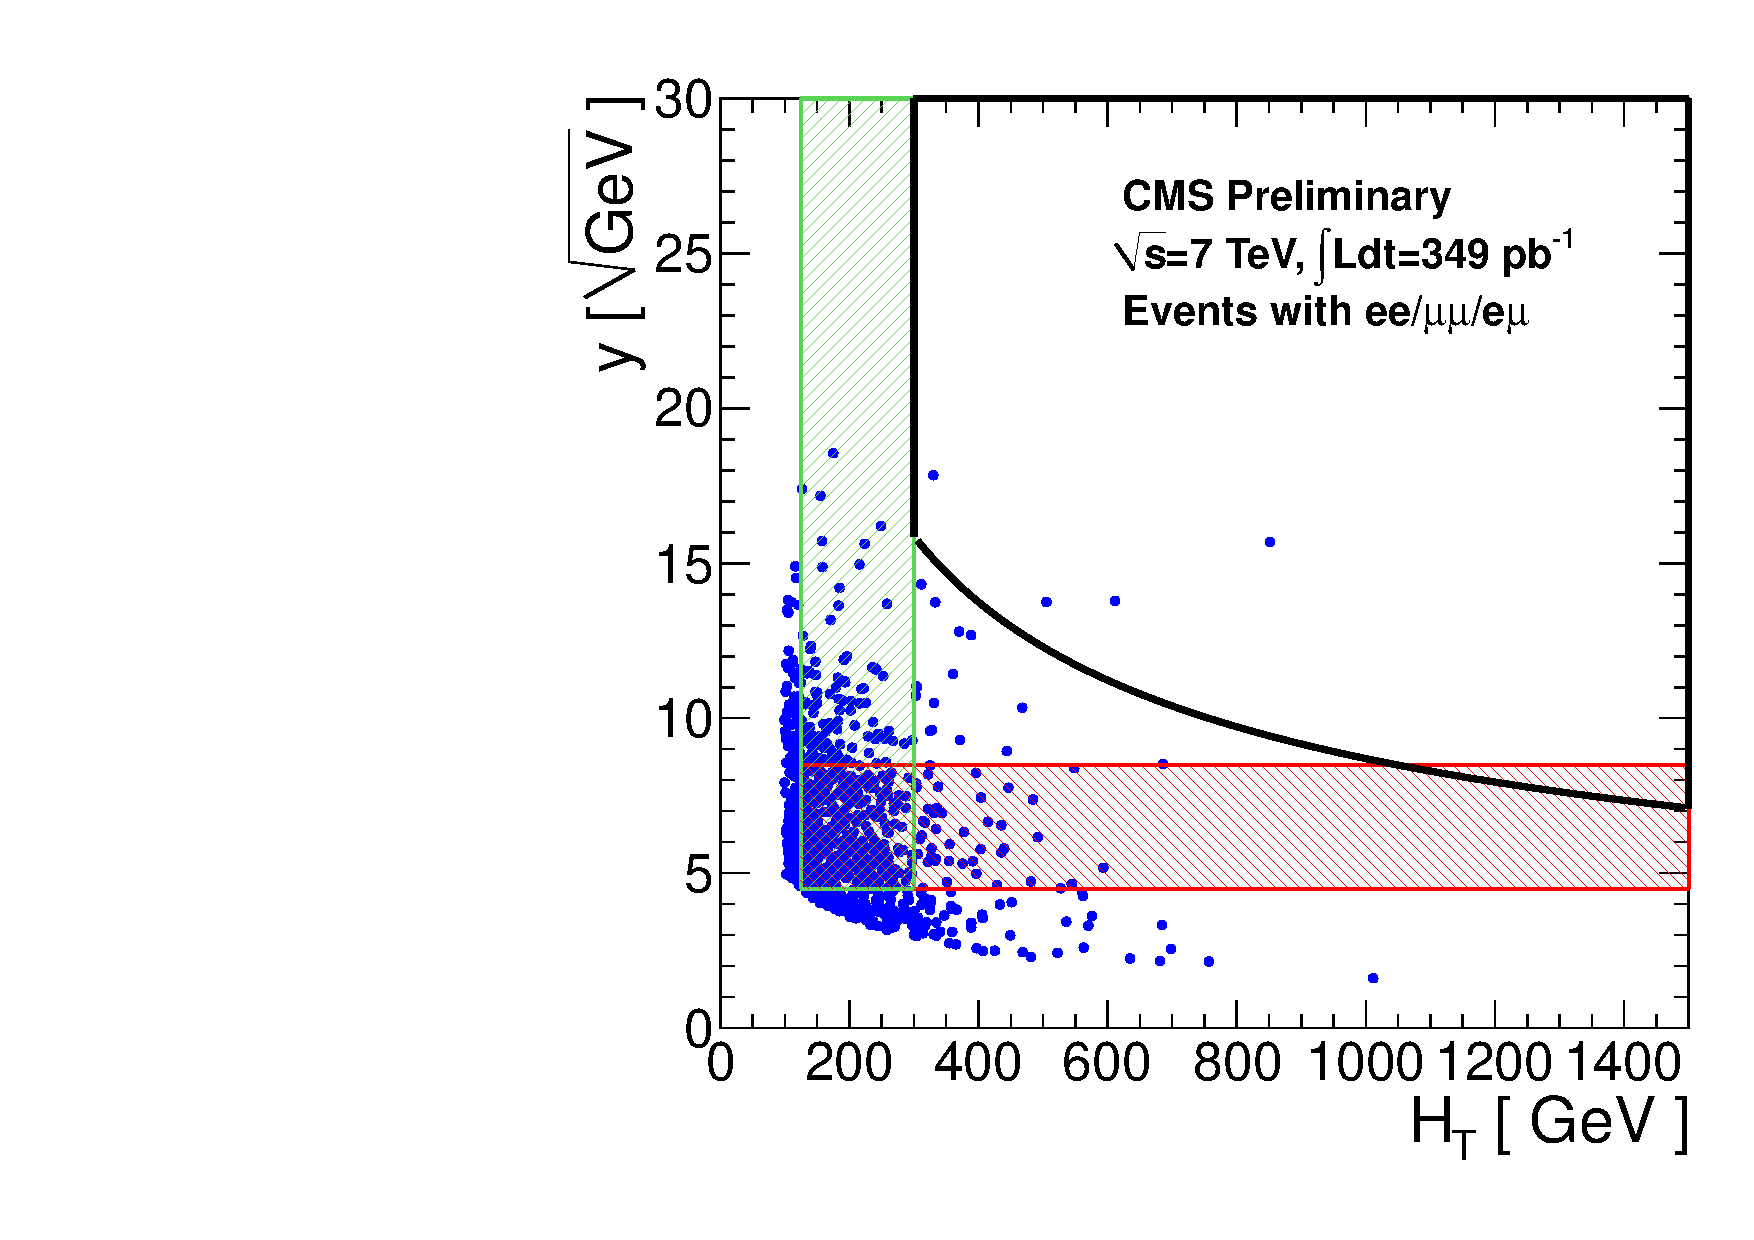
\includegraphics[width=0.48\linewidth]{plots/abcdprime_349pb_highmet.pdf}
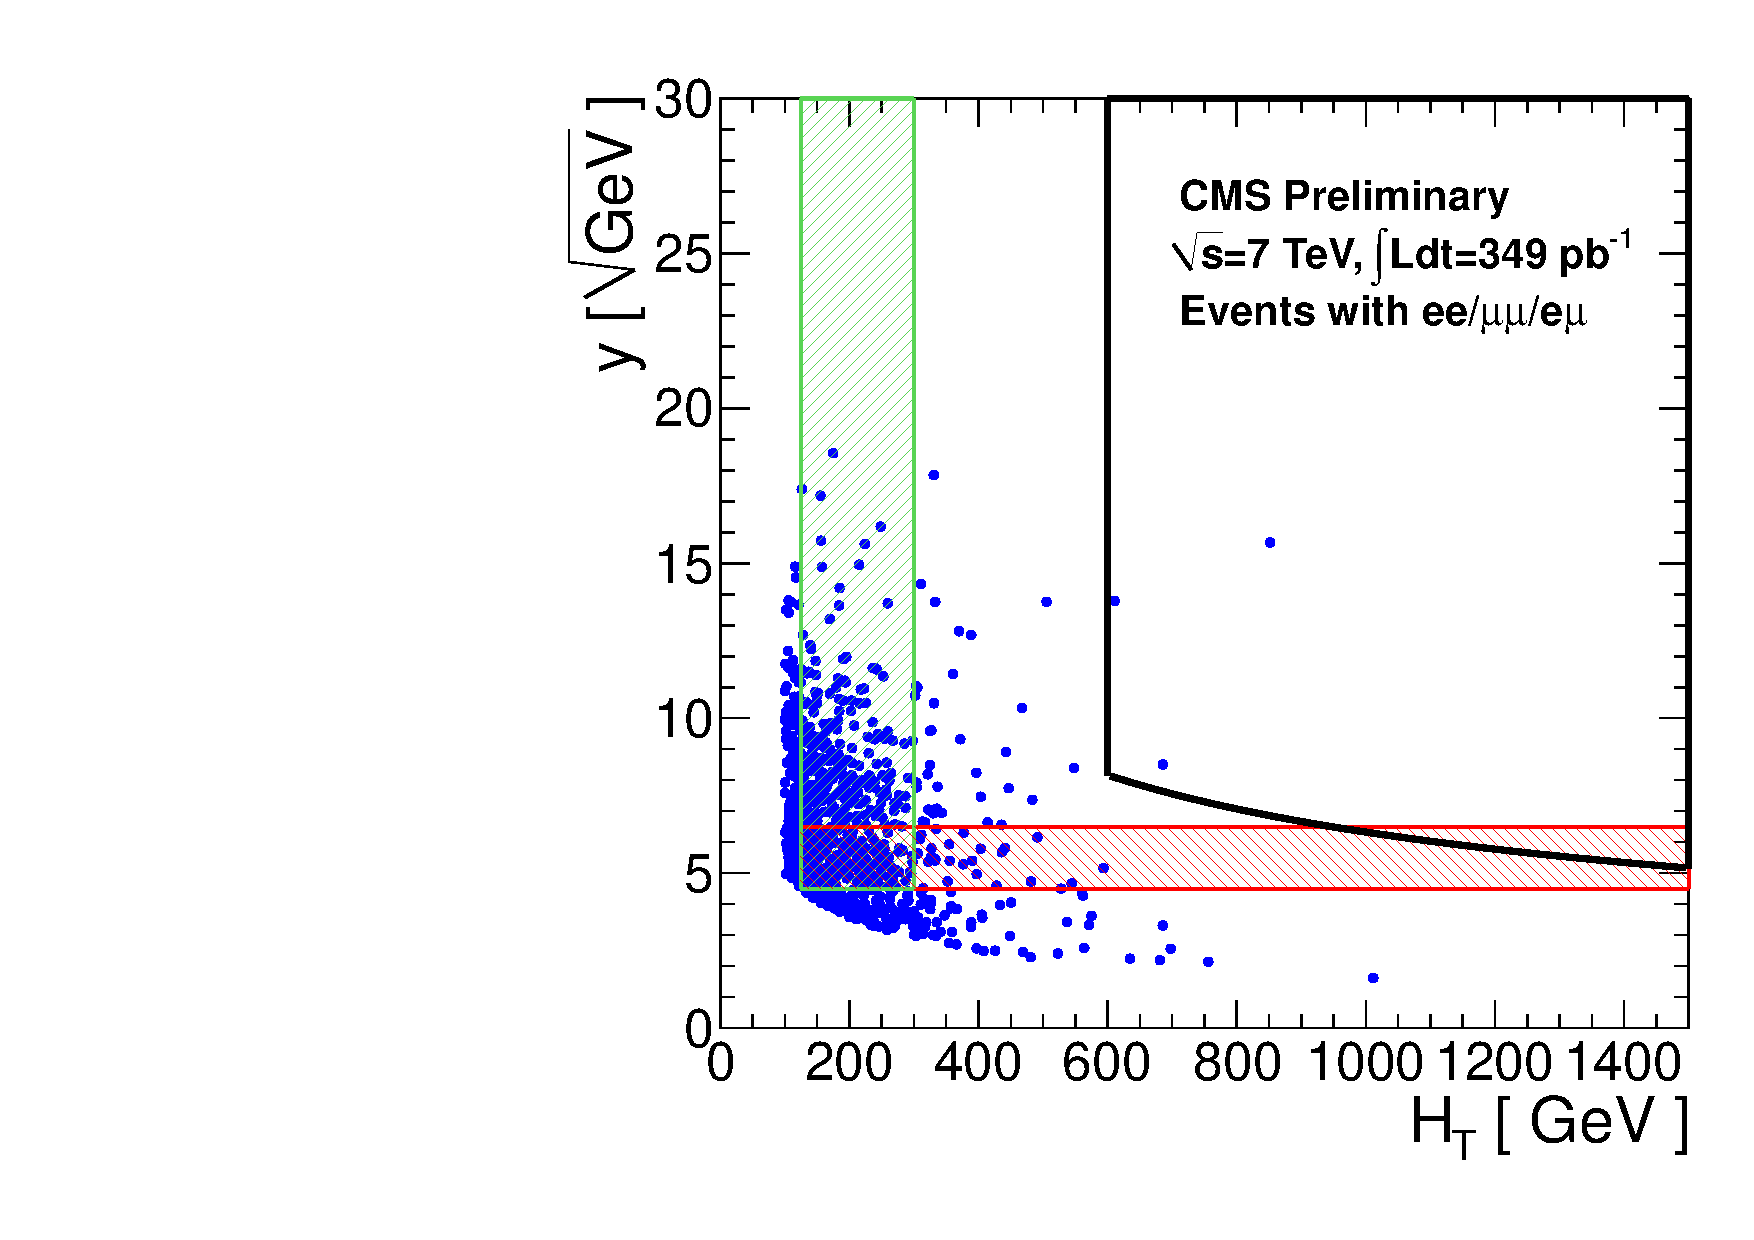
\includegraphics[width=0.48\linewidth]{plots/abcdprime_349pb_highht.pdf}
\caption{\label{fig:abcdprimedata}\protect 
Distributions of $y$ vs. \Ht\ in data. The signal regions \met\ $>$ 275 GeV, \Ht\ $>$ 300 GeV (left)
and \met\ $>$ 200 GeV, \Ht\ $>$ 600 GeV (right) are indicated with thick black lines. 
The $f(y)$ and $g(H_T)$ 
functions are measured using events in the green and red shaded areas, respectively.
}
\end{center}
\end{figure}

\subsection{Background estimate from the $P_T(\ell\ell)$ method}
\label{sec:victoryres}

We begin by extracting the value of the \met\ acceptance scaling factor $K$ from data,
for the \Ht\ control region 125--300 GeV and for the 2 signal regions \Ht\ $>$ 300 and
\Ht\ $>$ 600 GeV. The quantity $1/K$ is the efficiency for events passing preselection
and falling in the given \Ht\ range to pass the requirement \ptll\ $>$ 50 GeV.
The values of $K$ extracted from data and \ttbar\ MC are given in Table~\ref{tab:K}.
For all 3 \Ht\ regions, the value of $K$ extracted from data agrees with the 
\ttbar\ MC prediction, but for the \Ht\ $>$ 600 GeV region the statistical uncertainty
in $K$ from data is $\sim$100\%. Therefore we use the value of $K$ extracted from
data for the control region 125--300 GeV and for the signal regions \Ht\ $>$ 300;
for the \Ht\ $>$ 600 GeV region we use $K$ from \ttbar\ MC.

For each signal region D, we count the number of events falling in the region D', which is defined
using the same requirements as D but switching the $y$ requirement to a $\ptll/\sqrt{H_T}$ requirement (2010 signal region)
or switching the \met\ requirement to a \ptll\ requirement (high \met\ and high \Ht\ signal regions).
We subtract off the expected DY contribution using the data-driven $R_{out/in}$ technique, using $R_{out/in} = 0.13 \pm 0.07$.
%{\color{red} \bf add plot justifying this value}. 
We then scale this yield by 2 corrections factors:
$K$, the \met\ acceptance correction factor, and $K_C$, the correction factor determined in Sec.~\ref{sec:datadriven}.
Our final prediction $N_P$ is given by:

\begin{center}
$ N_P = (N(D')-N(DY)) \times K \times K_C$,
\end{center}

as summarized in Table~\ref{tab:victory}, and displayed in Figs.~\ref{fig:vic1}-\ref{fig:vic3}.
We also perform the \ptll\ method in the \Ht\ sideband region 125--300~GeV, as a validation of the technique in a high statistics
sample which is expected to be dominated by background. The results are summarized in Table~\ref{tab:victorycontrol}
and displayed in Fig.~\ref{fig:victorycontrol}.
The prediction is extractedd for the requirement $y > 8.5$~GeV$^{1/2}$ corresponding to the 2010 signal region, as well as
for \met\ $>$ 200 GeV corresponding to the high \Ht\ signal region. In both cases, we observe good agreement between
the predicted and observed yields.


\begin{table}[h!]
\begin{center}
\caption{\label{tab:K}
Summary of the \met\ acceptance scaling factor $K$, extracted from data and \ttbar\ MC.}
\vspace{.25cm}
\begin{tabular}{lccccc}
\hline
region                                    &  data              &   \ttbar\ MC      \\
\hline
control region: 125 $<$ \Ht\ $<$ 300 GeV  &  1.68 $\pm$ 0.14   &   1.67 $\pm$ 0.03 \\
signal region: \Ht\ $>$ 300 GeV           &  1.45 $\pm$ 0.29   &   1.50 $\pm$ 0.06 \\
signal region: \Ht\ $>$ 600 GeV           &  1.12 $\pm$ 1.19   &   1.32 $\pm$ 0.20 \\
\hline
\end{tabular}
\end{center}
\end{table}


\begin{table}[h!]
\begin{center}
\caption{\label{tab:victory}
Summary of results of the dilepton $p_{T}$ template method applied to the 3 signal regions.
The quantities indicated in the table are discussed in the text.
The quoted statistical uncertainty in the prediction $N_P$ is due to
that of $N(D')$, the quoted systematic uncertainty includes that of $N(DY)$, $K$, and $K_C$.
%{\bf K and KC taken from MC, do we want to take K and/or KC from data? }
%{\bf Need to add jet/met uncertainty here}
%{\color{red} \bf CURRENTLY USING 30\% UNCERTAINTY ON K_C IN 2010 REGION, WHICH IS WHAT WE HAD LAST YEAR (NEED TO REPEAT JET/MET UNCERTAINTIES?).}
%{\color{red} \bf FOR HIGH Y/HIGH HT REGION, TAKING SYST UNCERTAINTY ON KC FROM MC STATS, WHICH IS PROBABLY DOMINANT}
}
\vspace{.25cm}
\begin{tabular}{lccccc}
\hline
Signal Region               &  $N(D')$   &   $N(DY)$         &          $K$   &   $K_C$        & $N_P$                                   \\
\hline
2010 signal region (UPDATE) &       9    &   0.8 $\pm$ 0.4   & 1.5 $\pm$ 0.3  & 1.4 $\pm$ 0.4  & 16.7 $\pm$ 6.1 (stat) $\pm$ 5.9 (syst)  \\
high \met\ signal region    &       3    &   0.5 $\pm$ 0.3   & 1.5 $\pm$ 0.3  & 1.5 $\pm$ 0.5  & 5.4 $\pm$ 3.8 (stat) $\pm$ 2.2 (syst)   \\
high \Ht\ signal region     &       1    &   0.0 $\pm$ 0.0   & 1.3 $\pm$ 0.2  & 1.3 $\pm$ 0.4  & 1.7 $\pm$ 1.7 (stat) $\pm$ 0.6 (syst)   \\
\hline
\end{tabular}
\end{center}
\end{table}


\begin{table}[h!]
\begin{center}
\caption{\label{tab:victorycontrol} 
Summary of results of the dilepton $p_{T}$ template method applied to the \Ht\ sideband control region 125--300 GeV.
The quantities indicated in the table are discussed in the text.
The quoted statistical uncertainty in the prediction $N_P$ is due to
that of $N(D')$, the quoted systematic uncertainty includes that of $N(DY)$ and $K_C$.
The predictions are compare with the observed yield $N_O$.
}
\vspace{.25cm}
\begin{tabular}{lcccccc}
\hline
Control Region                                   &  $N(D')$   &   $N(DY)$        &  $K$          &   $K_C$          & $N_P$                                     & $N_O$ \\ 
\hline                                           
125 $<$ \Ht\ $<$ 300~GeV, $y >$ 8.5~GeV$^{1/2}$  &     54      &  2.6 $\pm$ 1.2   & 1.7 $\pm$ 0.1 & 1.4 $\pm$ 0.1    & 120.9 $\pm$ 17.3 (stat) $\pm$ 13.6 (syst) & 110   \\
125 $<$ \Ht\ $<$ 300~GeV, \met\ $>$ 200 GeV     &      4      &  1.0 $\pm$ 0.5   & 1.7 $\pm$ 0.1 & 1.3 $\pm$ 0.2    &   6.5 $\pm$  4.4 (stat) $\pm$  1.6 (syst) &   6   \\
\hline
\end{tabular}
\end{center}
\end{table}



\begin{figure}[h!]
\begin{center}
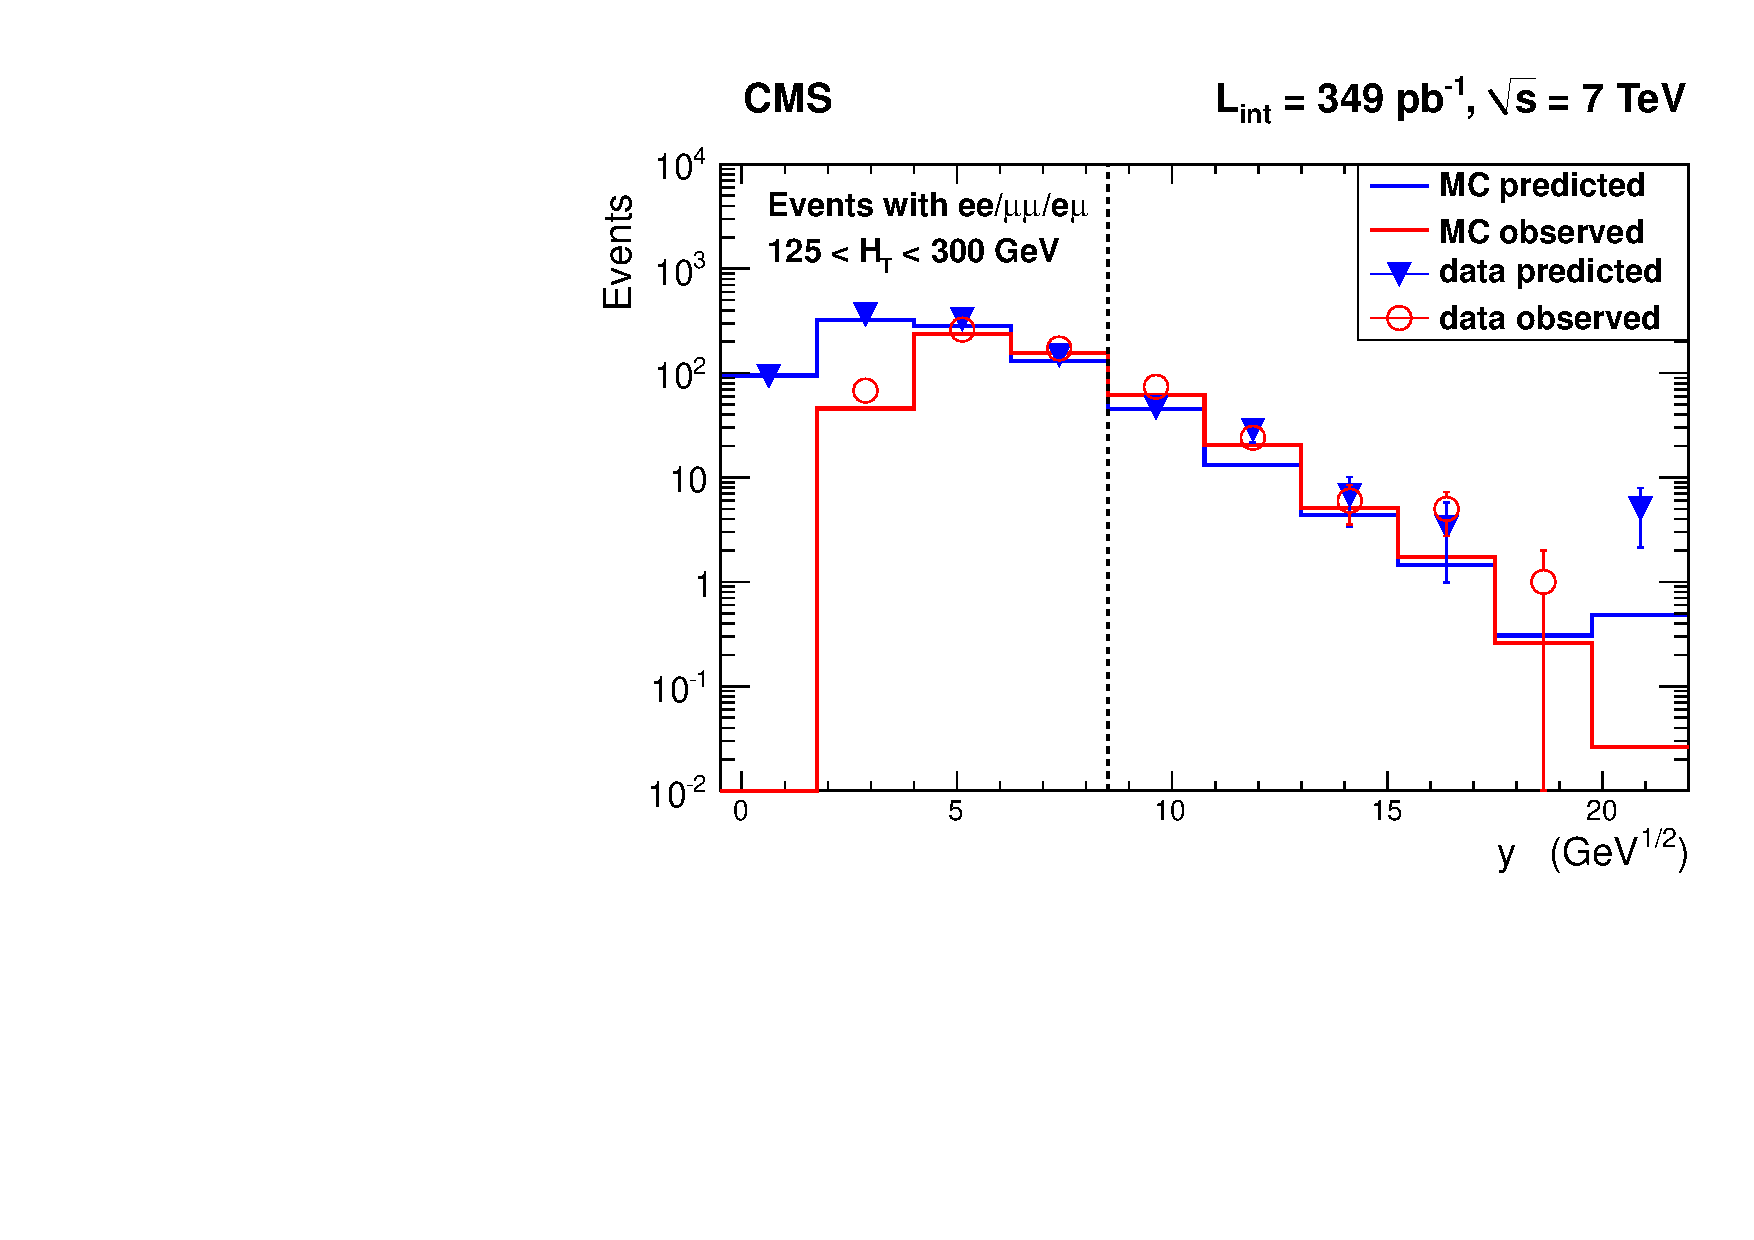
\includegraphics[width=0.48\linewidth]{plots/victory_y_control_349pb.pdf}
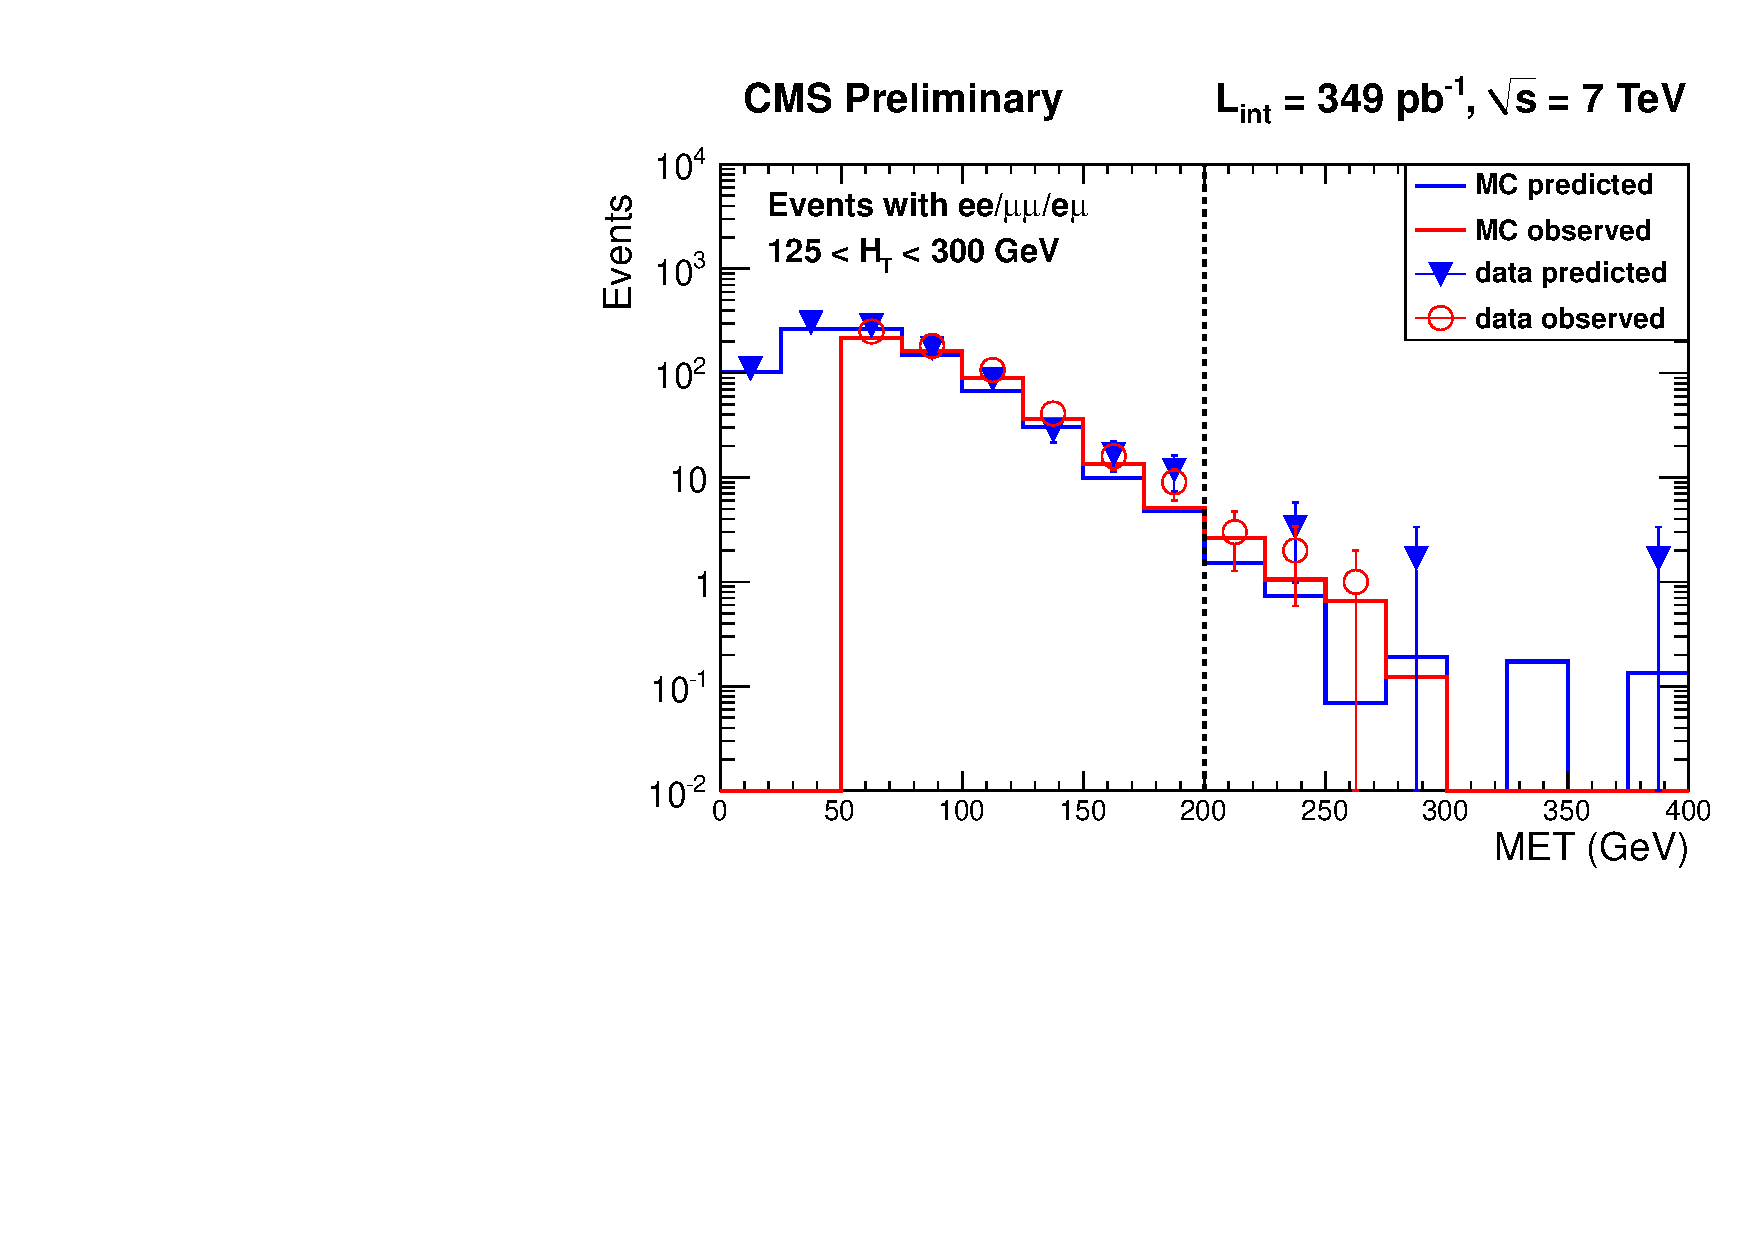
\includegraphics[width=0.48\linewidth]{plots/victory_met200_control_349pb.pdf}
\caption{\label{fig:victorycontrol}\protect 
Results of the \ptll\ method in the \Ht\ sideband region 125-300 GeV.
Left:  distributions of $\ptll/\sqrt{H_T}$ (predicted) and $y$ (observed) for 
SM MC and data. The vertical dashed lines indicate the requirement $y > 8.5$~GeV$^{1/2}$),
corresponding to the 2010 signal region.
Right: distributions of \ptll\ (predicted) and \met\ (observed) for 
SM MC and data. The vertical dashed lines indicate the requirement \met\ $>$ 200 GeV,
corresponding to the high \Ht\ signal region.
}
\end{center}
\end{figure}


\begin{figure}[h!]
\begin{center}
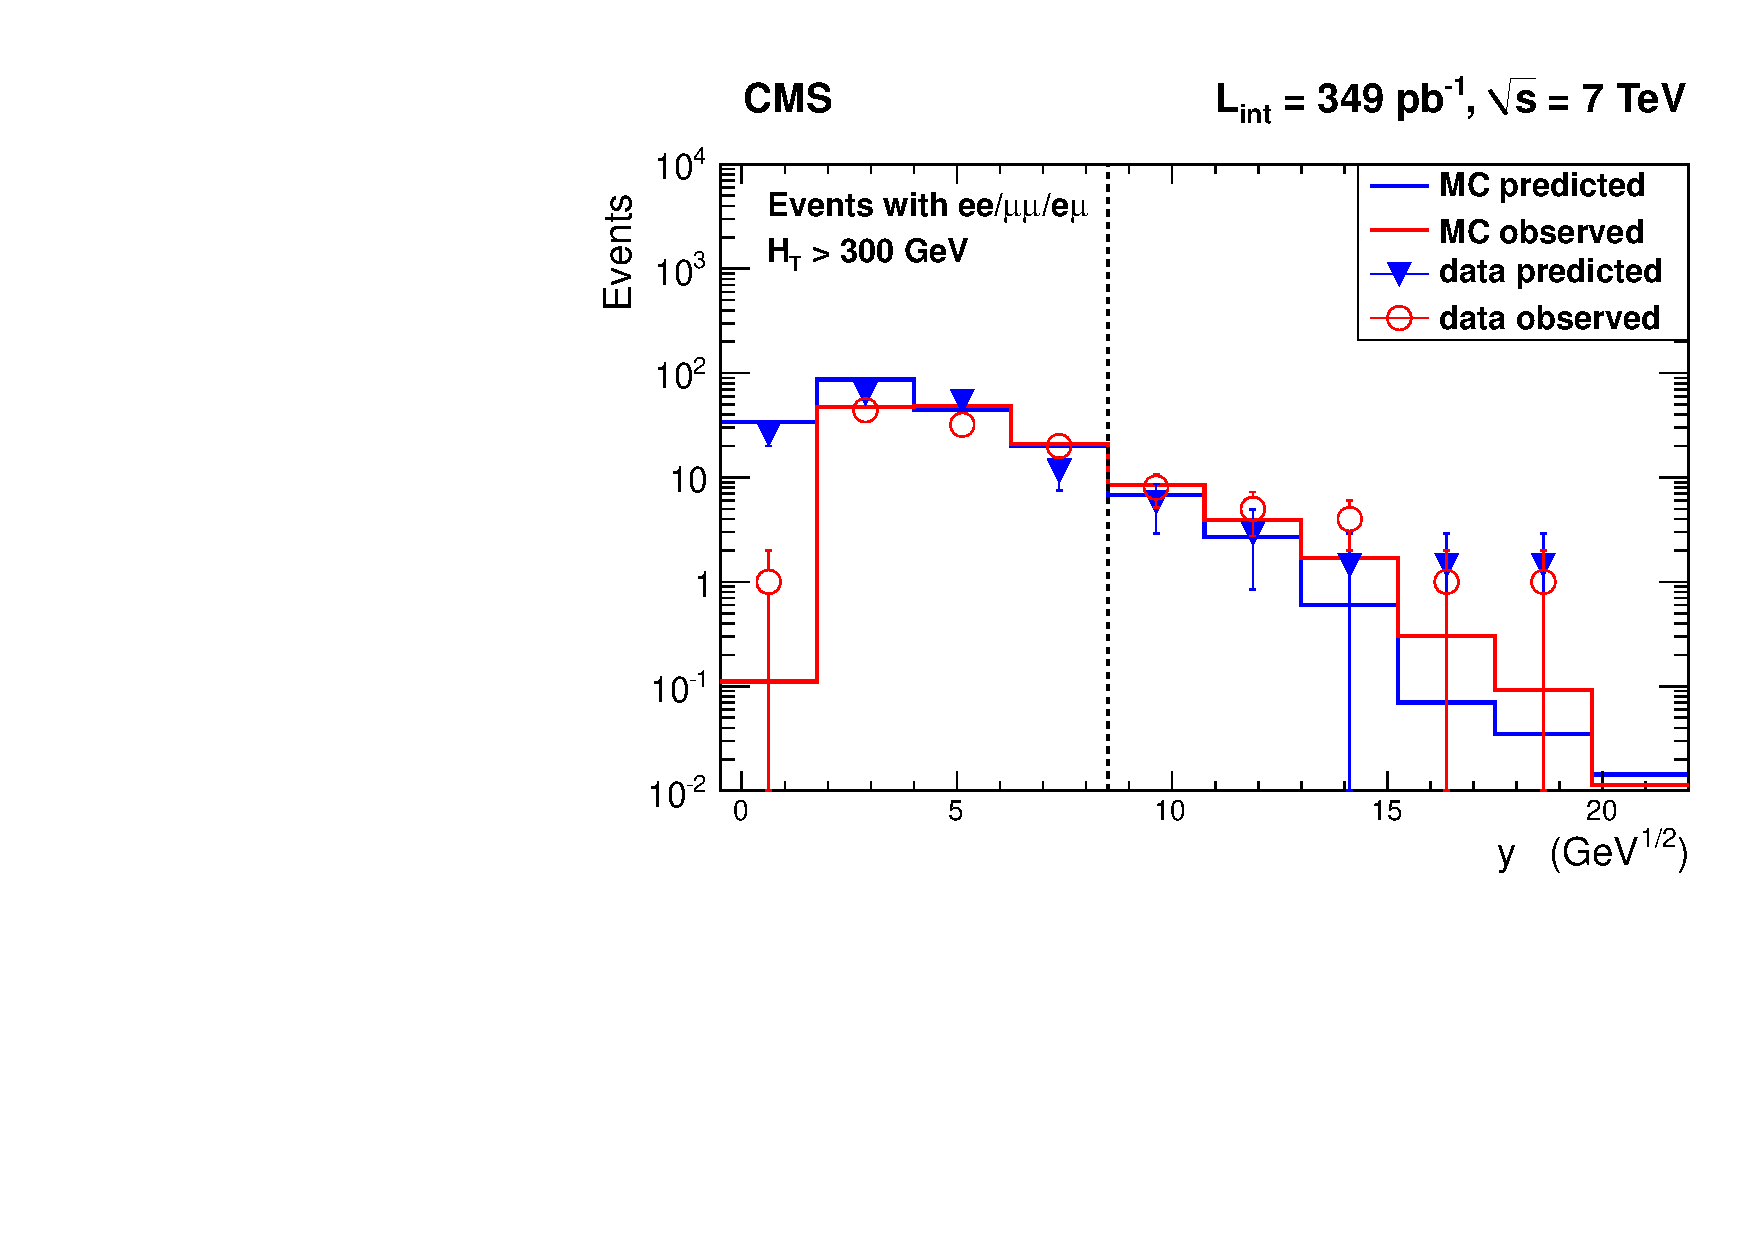
\includegraphics[width=0.6\linewidth]{plots/victory_y_ht300_349pb.pdf}
\caption{\label{fig:vic1}\protect 
Distributions of $\ptll/\sqrt{H_T}$ (predicted) and $y$ (observed) for 
SM MC and data, for the \Ht $>$ 300 GeV. 
The vertical dashed lines indicate the requirement $y > 8.5$~GeV$^{1/2}$ corresponding to the 2010 signal region.
}
\end{center}
\end{figure}

\begin{figure}[h!]
\begin{center}
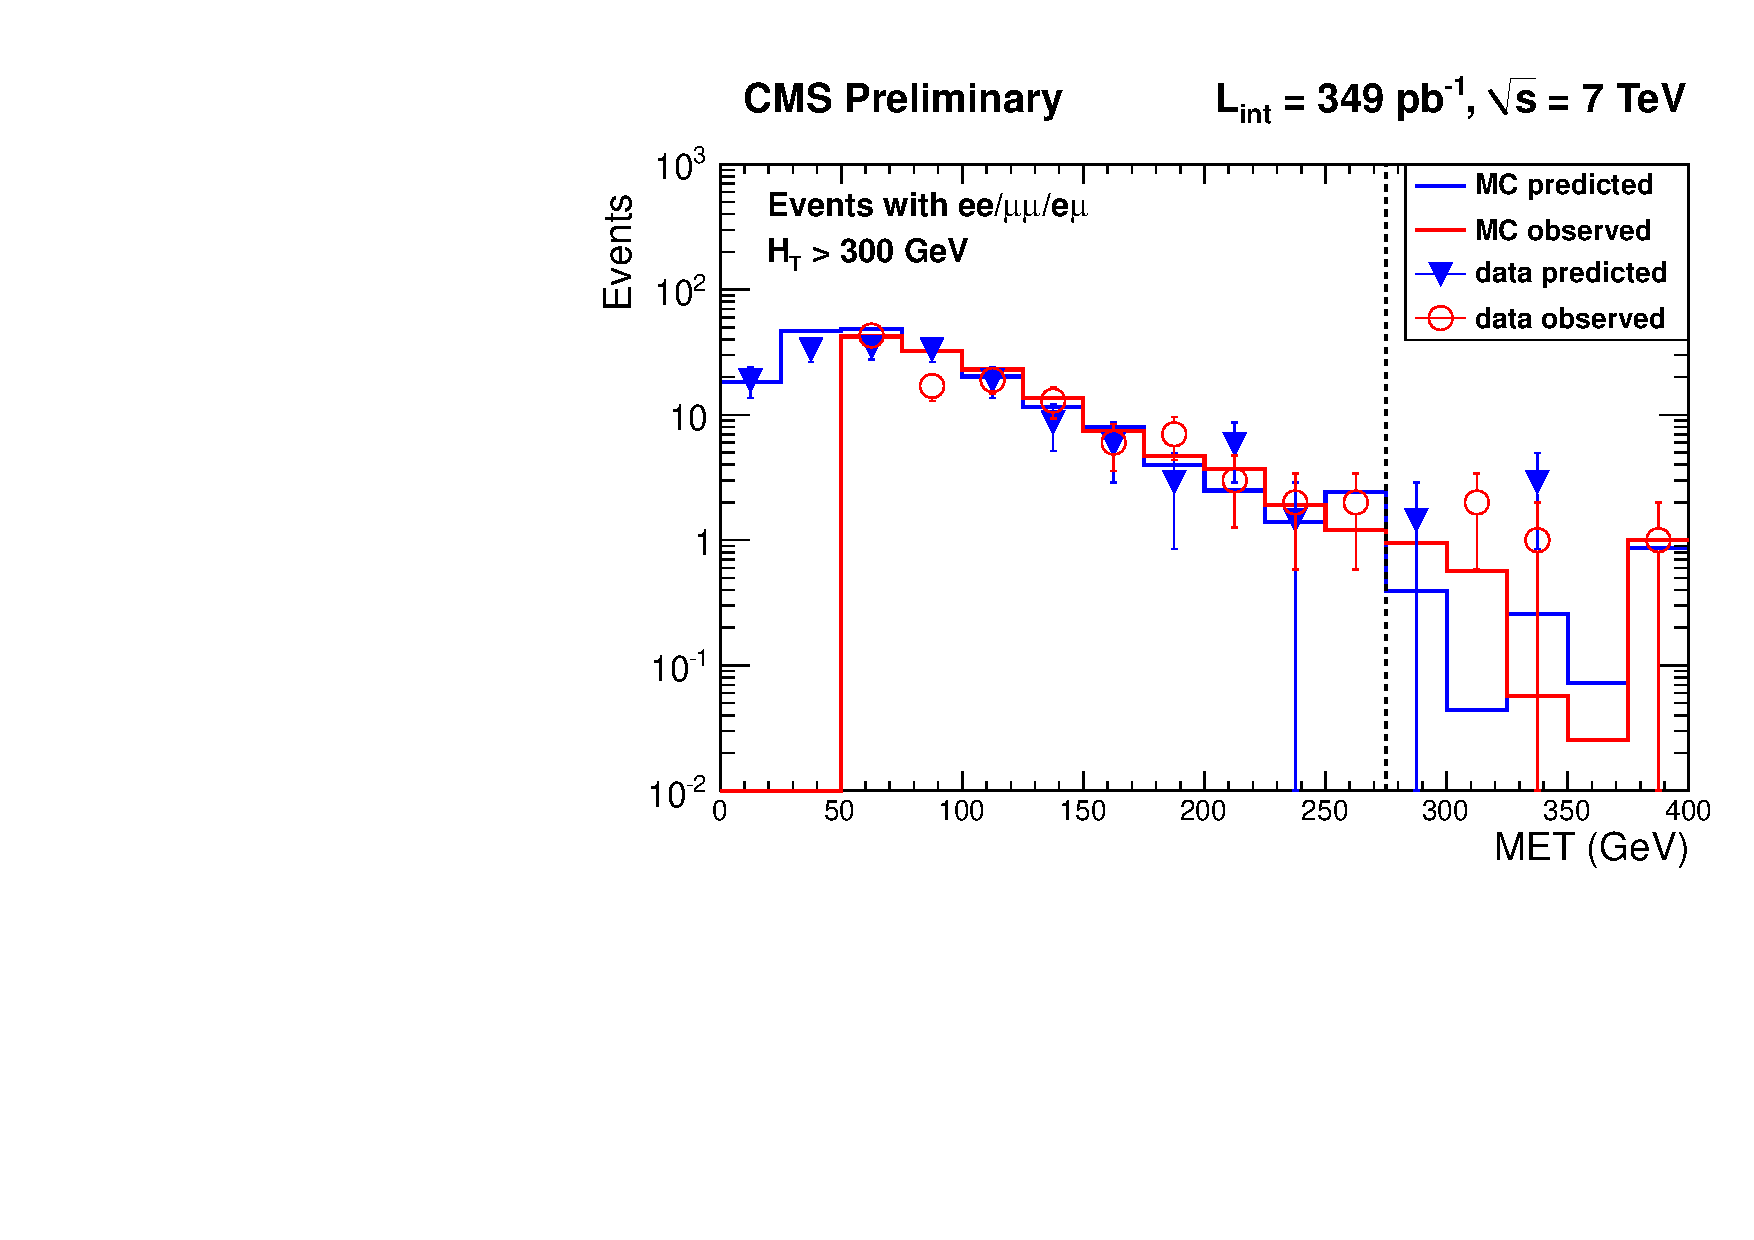
\includegraphics[width=0.6\linewidth]{plots/victory_met275_ht300_349pb.pdf}
\caption{\label{fig:v2}\protect 
Distributions of \ptll\ (predicted) and \met\ (observed) for 
SM MC and data, for the region \Ht $>$ 300 GeV. 
The vertical dashed lines indicate the requirement \met\ $>$ 275 GeV, corresponding to the high \met\ signal region.
}
\end{center}
\end{figure}

\begin{figure}[tbh]
\begin{center}
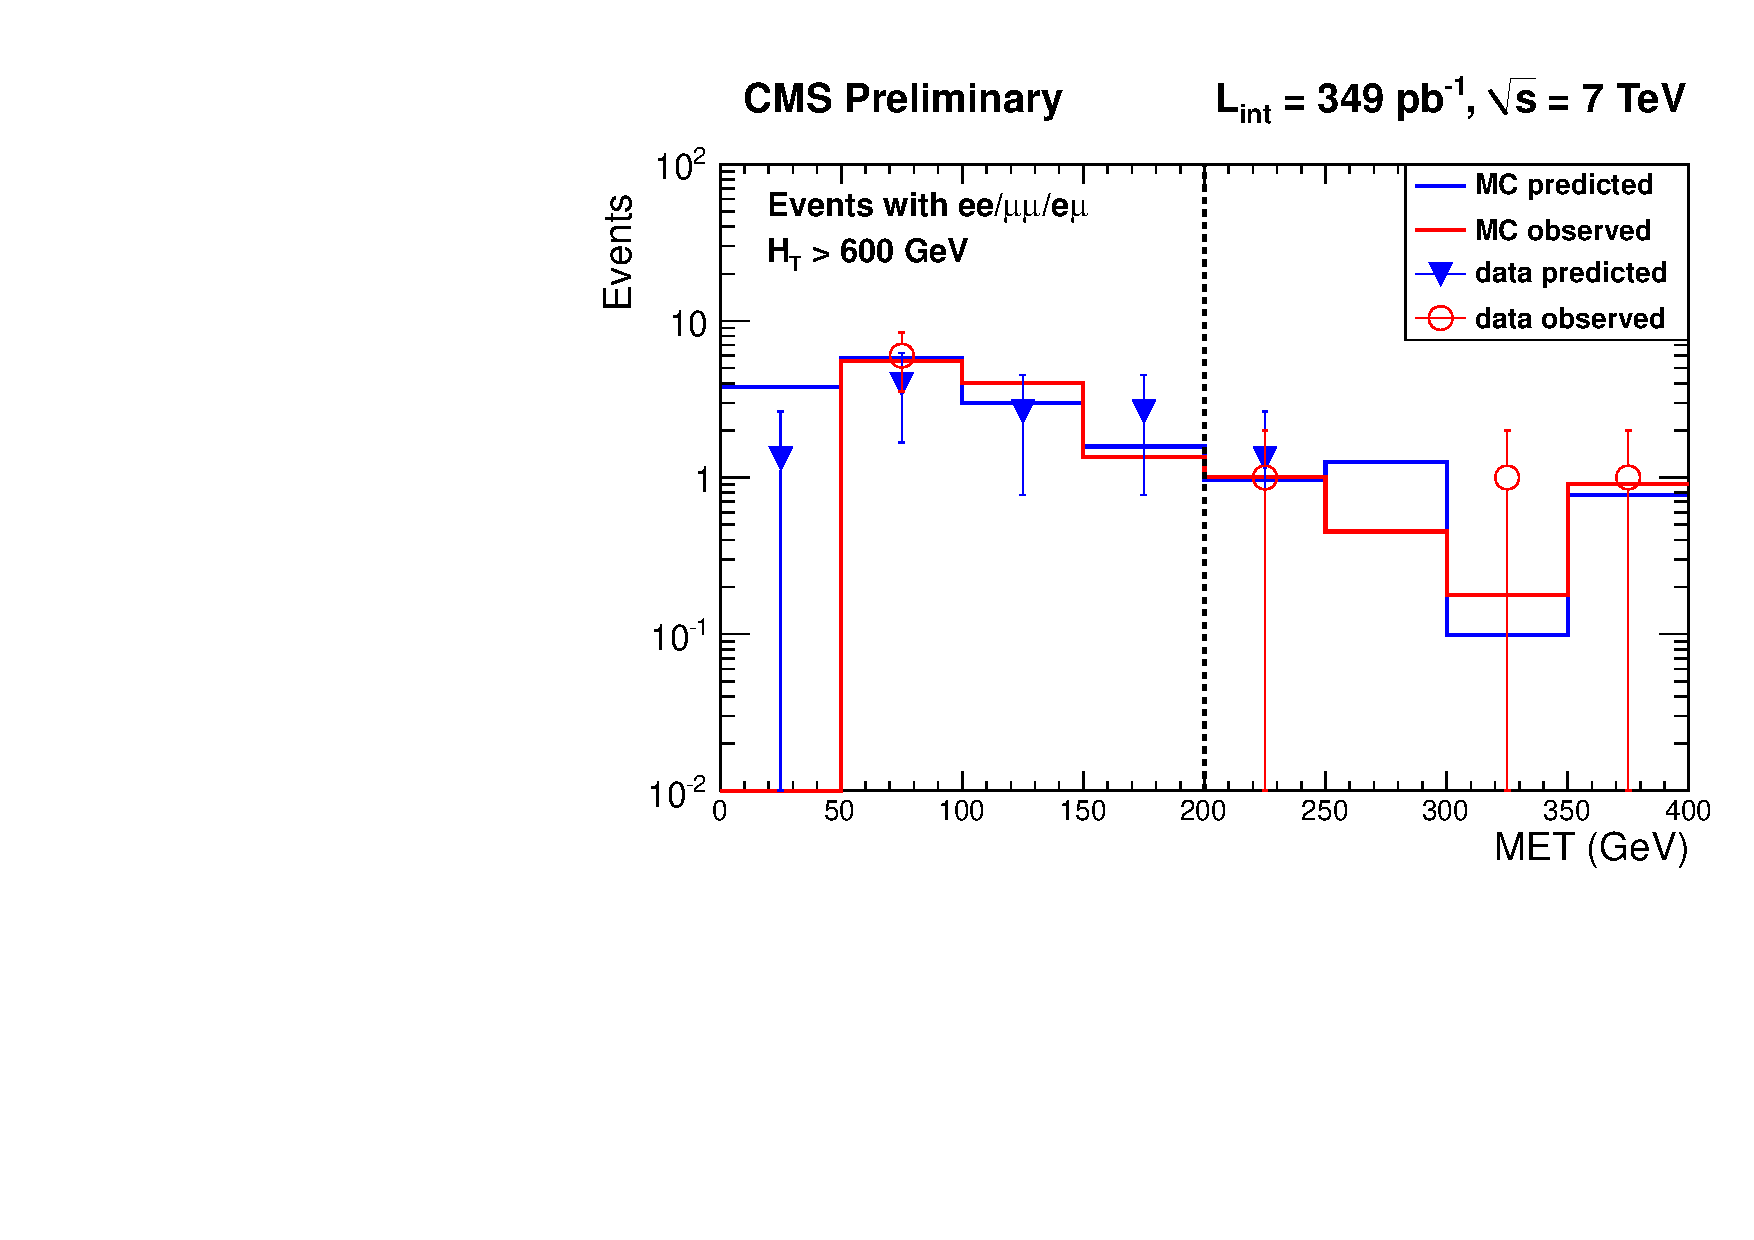
\includegraphics[width=0.6\linewidth]{plots/victory_met200_ht600_349pb.pdf}
\caption{\label{fig:vic3}\protect 
Distributions of \ptll\ (predicted) and \met\ (observed) for 
SM MC and data, for the region \Ht $>$ 600 GeV. 
The vertical dashed lines indicate the requirement \met\ $>$ 200 GeV, corresponding to the high \Ht\ signal region.
}
\end{center}
\end{figure}

\clearpage

\subsection{Background estimate from OF subtraction}
\label{sec:ofres}

The results of the OF subtraction technique applied to the high \pt\ dilepton trigger sample are summarized in Table~\ref{tab:ofres}. 
We evaluate the quantity $\Delta = R_{\mu e}N(ee) + \frac{1}{R_{\mu e}}N(\mu\mu) - N(e\mu)$ with $R_{\mu e} = 1.12 \pm 0.05$
extracted from the ratio of $Z \to \mu^+\mu^-$ vs. $Z \to e^+e^-$ events in data.
We perform the OF subtraction first in the preselection region, and find $\Delta$ consistent with 0, as expected.
We then perform the OF subtraction in all 3 signal regions, and do not observe any excess of same-flavor vs. opposite-flavor events.
We do not correct the value of $\Delta$ for contributions from fake leptons; instead, we assess on uncertainty based on
the results of Sec.~\ref{sec:dyFR}.

\begin{table}[hbt]
\begin{center}
\caption{\label{tab:ofres} Summary of results for the OF subtraction technique. 
The quantity $\Delta = R_{\mu e}N(ee) + \frac{1}{R_{\mu e}}N(\mu\mu) - N(e\mu)$ is quoted with $R_{\mu e} = 1.12 \pm 0.05$.
The quoted systematic uncertainty corresponds to that of $R_{\mu e}$ and the contribution from fake leptons. 
The $e\mu$ yields differ from those previously quoted because the $Z$ mass veto is included here.
}
\vspace{.25cm}
\begin{tabular}{l|ccc|c}
\hline
region                   &  $N(ee)$ & $N(\mu\mu)$ & $N(e\mu)$  &  $\Delta$   \\ 
\hline
preselection region      &      193 &         201 &      394   &    2.0 $\pm$ 28 (stat) $\pm$ 1.8 (syst) \\    
2010 signal region       &        4 &           4 &        9   &   -0.9 $\pm$ 4.2 (stat) $\pm$ 0.6 (syst)  \\
high \met\ signal region &        2 &           0 &        1   &    1.3 $\pm$ 1.9 (stat) $\pm$ 0.5 (syst)  \\
high \Ht\ signal region  &        1 &           0 &        1   &    0.1 $\pm$ 1.5 (stat) $\pm$ 0.5 (syst)  \\
\hline
\end{tabular}
\end{center}
\end{table}

For the dilepton-\Ht\ trigger sample, we observe only 1 event in the 2010 signal region, consistent with MC expectations,
and no events in either the high $y$ or high \Ht\ signal regions. In the case of an excess of events at low lepton \pt,
we will perform the OF subtraction technique of Sec.~\ref{sec:oflowpt}.

% \clearpage
\subsection{Summary of results}

A summary of our results is presented in Table~\ref{tab:results}. In all 3 signal regions, we observe reasonable agreement
between the observed yields and the predictions from MC and data-driven background estimates. We therefore do not observe
evidence for an excess of events above SM expectations. After assessing systematic uncertainties in Sec.~\ref{sec:systematics},
we proceed to set upper limits on the non-SM contributions to the signal regions in Sec.~\ref{sec:limits}.

\begin{table}[hbt]
\begin{center}
\caption{\label{tab:results} 
Summary of the observed and predicted yields in the 3 signal regions. MC errors are statistical only. The systematic uncertainty on the ABCD
and \ptll\ method is from the scaling factors from MC closure only. 
%{\bf need to put additional uncertainties, for example jet/met scale.}
For the OF subtraction, the quantity $\Delta = R_{\mu e}N(ee) + \frac{1}{R_{\mu e}}N(\mu\mu) - N(e\mu)$ is quoted; the systematic uncertainty
here is from the ratio of muon to electron selection efficiencies and from the contribution from fake leptons.
}
\vspace{.25cm}
\begin{tabular}{l|c|c|c}
\hline
                                       &  2010 signal region                       &   high \met\ signal region             &  high \Ht\ signal region              \\ 
\hline
Observed yield                         &         19                                &                        4               &                        3              \\
\hline
MC prediction                          &    14.5 $\pm$ 1.4                         &            2.6 $\pm$ 0.8               &            2.5 $\pm$ 0.8              \\
ABCD prediction                        &    12.7 $\pm$ 2.4 (stat) $\pm$ 2.5 (syst) &                                        &                                       \\
ABCD' prediction                       &    12.8 $\pm$ 2.9 (stat) $\pm$ 2.6 (syst) & 1.2 $\pm$ 0.4 (stat) $\pm$ 0.5 (syst)  & 0.0 $\pm$ 0.6 (stat) $\pm$ 0.3 (syst) \\
\ptll\ prediction                      &    16.7 $\pm$ 6.1 (stat) $\pm$ 5.9 (syst) & 5.4 $\pm$ 3.8 (stat) $\pm$ 2.2 (syst)  & 1.7 $\pm$ 1.7 (stat) $\pm$ 0.6 (syst) \\
\hline
OF subtraction ($\Delta$)              &    -0.9 $\pm$ 4.2 (stat) $\pm$ 0.6 (syst) & 1.3 $\pm$ 1.9 (stat) $\pm$ 0.5 (syst)  & 0.1 $\pm$ 1.5 (stat) $\pm$ 0.5 (syst) \\
\hline
\end{tabular}
\end{center}
\end{table}
